\chapter{Introduction and Background}

\section{Introduction}
In Pakistan, the vast majority of industrial manufacturing is currently done through manual labor. This is particularly true for assembly lines, where products are packaged and palletized by hand, such as in the project’s case study: the microwave line at a Dawlance assembly plant. Workers have to lift heavy microwaves (on average, 20kg), place them inside boxes carefully, insert expanded polystyrene (EPS) pieces for packing, seal the flaps with tape, and then finally lift and orient the final product onto a pallet, stacking at various heights, as shown in Fig.\ref{fig:process}. This action is performed daily for hours on end.

\begin{figure}[H]
    \centering
    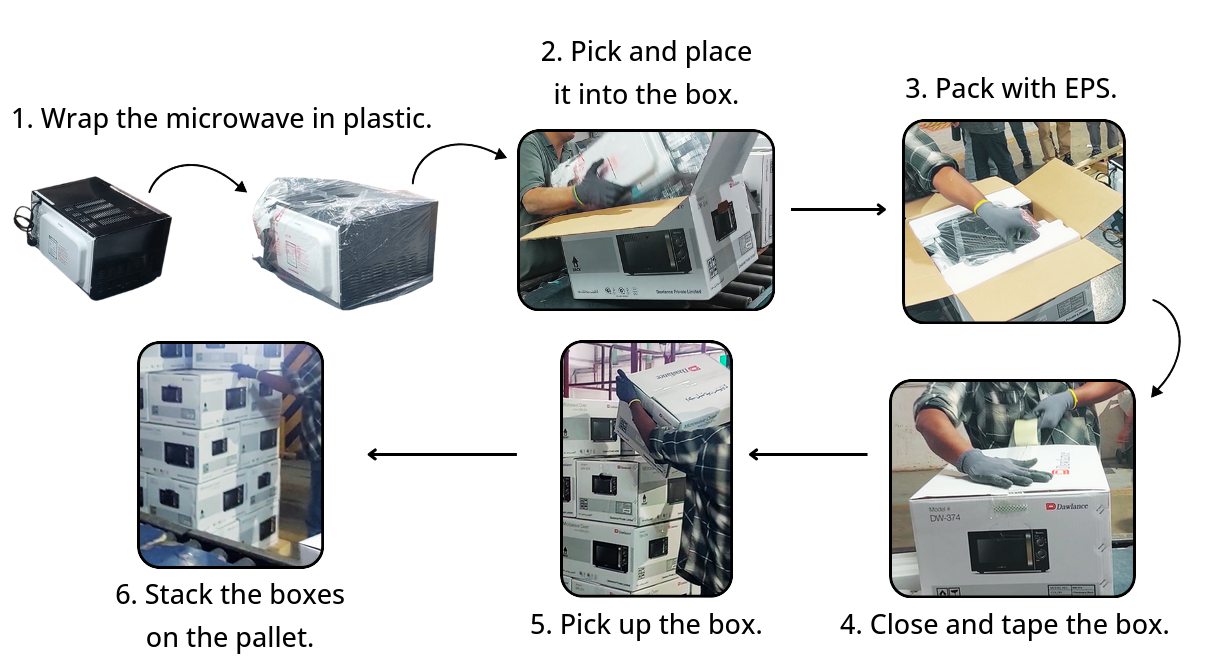
\includegraphics[ width=\linewidth]{figures/process.png}
    \caption{A flowchart demonstrating the process at the plant.}
    \label{fig:process}
\end{figure}

To evaluate the ergonomic risk of this process, the NIOSH Lifting Index is employed, which is a metric that estimates the physical stress by calculating the ratio of the actual load weight to the recommended weight limit. \cite{niosh_rnle} This turns out to be 3.1; for context, a score above 3.0 means that the process must be redesigned, because nearly all workers performing this task have a high probability of developing long-term disorders or injuries, even if they are highly trained and maintaining proper positioning etiquette. The analysis of this calculation is consistent with the findings of broad industry studies, which suggest that manual palletizing is dangerous because of the high risk of developing musculoskeletal disorders (LBDs). \cite{gallagher2015effects, yildirim2014identifying}

This is not the only concern. Workers are prone to fatigue, which means that the chances of damaging a product increases over time. Examples include crumpling the corners of a cardboard box while palletizing, inadvertently dropping the microwave roughly into the box, and creating minor errors in the stacking operation, thus weakening the overall interlocking structure on the pallet. Major product damage means that the product is discarded, creating waste, so even if minor damage passes quality tests, potential customers are influenced negatively, harming sales.

Due to these issues extending to general manufacturing industries, many companies have turned to fully automated solutions such as installing articulated robots. While this is an effective solution for global giants, the feasibility fades for local Pakistani markets, largely due to the capital and maintenance costs associated with importing these robots. ``A basic collaborative robot starts around \$25,000, while full industrial automation systems can reach \$500,000 or more." \cite{standardbots2025costs} Moreover, for maintenance, the expertise for handling the proprietary software is not present, since the manufacturers for the robots are not in the country, so this is an unsustainable solution. This leaves room for local engineering innovation, which has been slow in Pakistan.

The solution would need to meet several requirements owing to the constraints of the microwave line. It needs to lift payloads of up to \SI{40}{kg} (this incorporates a safety factor) within a 30-second takt time, operate along with human workers, and be wholly manufactured from locally sourced components within a budget of Rs. 1.8 million. Moreover, this solution must be maintainable by Dawlance's engineering staff to eliminate dependence on foreign expertise. 

Furthermore, the development of a solution is complicated by three major challenges. A primary issue is the conflict between optimizing production speed and reducing complexity of dexterous manipulation. If the entire pipeline is to be automated, a large amount of time would be invested in fine manipulation for handling light objects, which a human worker would perform much faster. To match that, the automated system would need highly powerful hardware, which is limited in Pakistan, particularly under a modest budget. Thus, a single automated system is unlikely to perform both heavy lifting and dexterous manipulation in a short time window.

Secondly, the robot needs to cover a few meters in each direction, creating a critical mechanical conflict between speed and rigidity. For example, lead screws are highly rigid, but the rotational speeds required to meet the cycle time cause dangerous mechanical whipping due to resonance. Belt drives are fast, but introduce hysteresis under heavy loads, while rack-and-pinion systems are heavy and demand greater structural integrity. Moreover, the latter two systems are backdrivable, which is a severe safety risk on the Z-axis as there would be no mechanical friction to prevent heavy microwaves from free-falling in case of power failure. So, the drive mechanisms must be carefully selected
and engineered to resolve this complex issue.

Finally, the end-effector design is conflicted between speed and security, because the payload (a boxed microwave) is heavy and has a smooth surface. For instance, vacuum systems allow for rapid picking, but may detach during sudden changes in acceleration or power loss. Meanwhile, mechanical grippers lock more securely, but need greater clearance and are generally slower. As a result, regardless of robot architecture, the design of the end-effector is not straightforward.

Altogether, this background context informed every major design decision in the project, which is elaborated on in the remaining chapters.

\section{Literature Review of Solutions}
This section outlines a survey of existing automation technologies for packaging and palletizing, followed by a systematic selection justification based on the specific constraints presented in the context of the project.

\subsection{Overview of Automation Technologies}

For pick-and-place tasks in industry automation, literature offers several robot architectures: SCARA, delta, parallel, articulated, and gantry robots. However, once the constraints of this project -- heavy payloads, large workspace, inexpensive manufacturing -- are taken into consideration, the literature is largely dominated by the presence of articulated robots, formally known as serial manipulators, and gantry robots.

Articulated robots are similar to the structure of a human arm, with a series of rotary joints covering X, Y, Z, and Yaw axes, optionally extending to Pitch and Roll to obtain control of all six degrees of freedom (DoF) in 3D space. Market analysis shows that articulated robots command 40\% of the global industrial robotics market share, which is the highest \cite{gminsights2024} and establishes them as the standard.

According to academic literature, the primary advantage of articulated robots is their flexibility when generating complex trajectories \cite{siciliano2016robotics}. Hence, these can function in unstructured environments requiring approaching from arbitrary angles. However, a trade-off is presented in its stiffness, which depends on its configuration. Research by Woolfrey et al.\ shows that the stiffness of the endpoint of an articulated arm is a function of its Jacobian matrix, so its ability to resist external forces varies greatly depending on the parameters of the matrix, which includes the extension of the arm and the joint angles \cite{woolfrey2024optimal}.

A second solution in academic literature is gantry robots, also known as Cartesian robots. These systems contain a structural frame where the axes of the end-effectors are controlled directly by linear actuators. Moreover, unlike articulated robots, which are cantilevered and must compensate for inertia and gravity, gantry carriages are supported at both ends on the frame. Because of this structural difference, gantry robots have a naturally high stiffness-to-weight ratio and superior stability over large workspaces; however, gantry robots have significantly lesser dexterity as a trade-off \cite{groover2016automation}.

Recent comparisons in industrial automation suggest that for applications requiring transfer of heavy payloads over extensive areas, gantry systems are more appropriate. Articulated arms demand large motors for greater reach due to their cantilevered design; in contrast, gantry workspaces can be expanded simply by an extension of the rail length, rendering them highly modular and scalable for packaging and palletizing operations \cite{bostelman2016survey}.

To further systematically evaluate these technologies for the constraints of the project, a comparison of key parameters is presented in Table \ref{tab:robot_comparison}.


\begin{table}[H]
    \centering
    \caption{Comparative Analysis of Articulated vs. Gantry Robots \cite{siciliano2016robotics, groover2016automation}}
    \label{tab:robot_comparison}
    \renewcommand{\arraystretch}{1.3}
    \begin{tabular}{@{}p{2.2cm} p{5.5cm} p{5.5cm}@{}}
        \toprule
        \textbf{Parameter} & \textbf{Articulated Robot} & \textbf{Gantry Robot} \\
        \midrule
        \textbf{Workspace} & Spherical/Cylindrical; limited by arm reach. & Rectangular prism; scalable by rail extension. \\
        \hline
        \textbf{Payload \& Stability} & Variable (Jacobian-dependent); cantilevered structure. & Constant; high stiffness due to frame support. \\
        \hline
        \textbf{Speed \& Precision} & High speed; precision decreases at max reach. & Moderate speed; high precision over large areas. \\
        \hline
        \textbf{Flexibility} & High (6-DoF); can approach from any angle. & Moderate (3-4 DoF); fixed vertical approach. \\
        \hline
        \textbf{Cost} & High upfront CAPEX; expensive proprietary parts. & Low; uses standard motors and structural profiles. \\
        \hline
        \textbf{Integration Complexity} & High; requires proprietary programming expertise. & Low; intuitive kinematics and open-source control. \\
        \bottomrule
    \end{tabular}
\end{table}

\subsection{System Selection Justification}

While articulated robots are ideal for established global enterprises, their feasibility diminishes for Small and Medium Enterprises (SMEs) in developing economies such as Pakistan. Urrea et al.\ notes that SMEs often face barriers to entry of articulated robots, including high implementation costs, incompatibility with legacy systems, and a shortage of technical expertise specialized to the systems \cite{urrea2024advances}. Beyond the initial capital expenditure, the lack of local manufacturing for proprietary articulated robot controllers means that industries are highly dependent on foreign supply chains. In contrast, the linear and modular nature of gantry systems permits fabrication using locally sourced components and microcontrollers, which addresses sustainability and maintenance.

Consequently, the gantry robot is selected as the viable option for the project. Packaging and palletization of microwaves is a structured task needing heavy lifting over a large constant area, instead of highly dexterous and complex 6-DoF manipulation. The gantry topology has greater payload capability than articulated arms due to its stable frame, which mitigates the need for inertia compensation and allows a relaxation of torque constraints from motors.

\subsection{Operational Paradigm}

Following selection of mechanical architecture, the operational paradigm must be defined. While Industry 4.0 recommended total automation of industrial tasks, recent trends have shifted towards a new industrial movement: Industry 5.0. This paradigm is defined by the European Commission as one that ``places the wellbeing of the worker at the centre of the production process'', with technology serving to assist humans, instead of replacing them \cite{breque2021industry5}.

This project adopts this human-centric approach. As automating dexterous tasks (wrapping plastic, inserting EPS blocks, minor positional adjustments, etc.) remains costly and offering poor returns compared to human labor, the system is designed for human-robot collaboration (HRC), where the robot handles hazardous heavy lifting, while team members carry out the remaining dexterous tasks. To ensure safety in this environment, the system design follows international standards: ISO 10218-1/2 lists the foundational safety requirements that industrial robots must adhere to, whereas ISO/TS 15066 provides the specifications for collaborative operations, such as limiting force and monitoring speed \cite{iso15066}. Thus, interaction between the gantry system and team members are ensured to be safe.

\section{Problem Statement and Objectives}
The main qualities identified to be addressed are worker safety, product quality, and process inefficiency. Hence, after deliberation with the Dawlance management, the project’s problem statement is defined as: \textbf{``How can we protect product quality and improve worker ergonomics through automation of microwave packaging and palletizing?''}

Within this problem statement lies the primary objective of designing, manufacturing, and testing a robotic system to perform the particularly physically demanding tasks to package and palletize microwaves at the end of an assembly line. Based on this, there are five major secondary objectives:

\begin{itemize}
    \item \textbf{Improve ergonomics.} In particular, bring the NIOSH Lifting Index value to a safe one below 1.0.
    \item \textbf{Maintain product quality.} As stated by the plant supervisor, the magnetron should be protected, and minor errors should be mitigated by the elimination of human mistakes due to fatigue.
    \item \textbf{Meet the production speed.} Currently, the takt time is 30s; the solution must be faster than this or at worst equal.
    \item \textbf{Be affordable.} Dawlance has requested that the project's Bill of Material remains under Rs 1.8 million.
    \item \textbf{Be flexible and reliable.} The system must accommodate all microwave models currently in production without failure. 
\end{itemize}


